
\chapter{METHODS AND RESULTS}

    This section consists of the simulation physics which are utilized and simulation results of X-cut  Z-cut EO modulators.
    
    There are  two simulation physics utilized one of them is to determine optical field mode in TFLN waveguide and it is called as \textit{Electromagnetics Wave, Frequency Domain (ewfd)}. The other physic utilized is \textit{Electrostatics (es)} to simulate static field distribution through gap area of CPW. 
    
    Firstly, simulation configurations are checked by realizing the geometry based on the paper \cite{21}.  The mode confinement and overlap with DC field distribution are derived from COMSOL 6.0. Then COMSOL-MATLAB Livelink is utilized in order to calculate overlap integral and $V_\pi$ voltage is calculated based on that value. After than that, another simulation was run for the modulator which Girish Karthik experimentally measured in the laboratory and results are compared. Finally, parametric simulations are done to observe how $V_\pi L$ value responds to these changes and to see how loss can be limiting factor to realize some of the modulator geometries. 


    \subsubsection{Verification of Simulation}

    Zhang et al. \cite{21} has calculated $V_\pi$ voltages for different thin film optical waveguides.  


    \begin{table}[h!]
        \centering
        \caption{X-cut and Z-cut TFLN modulator dimensions and calculated $V_{\pi}.L$ values by Zhang et al. [21]}
        \begin{tabular}{|c|c|c|}
            \hline
            \textbf{Label} & \textbf{X-Cut LN} & \textbf{Z-Cut LN} \\
            \hline
            Structure & 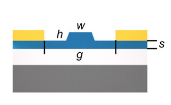
\includegraphics[width=0.2\textwidth]{x-cut-paper.PNG} & 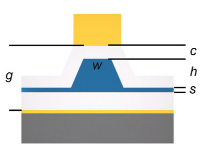
\includegraphics[width=0.2\textwidth]{z-cut-paper.PNG} \\
            \hline
            Slab thickness (s)  & 200 nm & 300 nm \\
            \hline
            Ridge height (h) & 400 nm & 1.2 $\mu m$ \\ 
            \hline
            Ridge width (w)& 770 nm & 800 nm\\
            \hline
            Cladding thickness (c)&  Parametric & 3.2 $\mu m$ \\
            \hline
            Metal gap (g) & $ 2\mu m$ & 700 nm\\
            \hline
            $V_{\pi}.L$ (push-pull) & 2.25 $V.cm$ & 2.6 $V.cm$\\
            \hline
        \end{tabular}
        \label{table:zhang-et-al}
    \end{table}

    In their study, they focused on all-LN x-cut rib waveguide desing and all-LN z-cut rib waveguide design with planar electrode, which is in line with the aim of this work.  

   
    %\begin{figure}
    %    \centering
    %    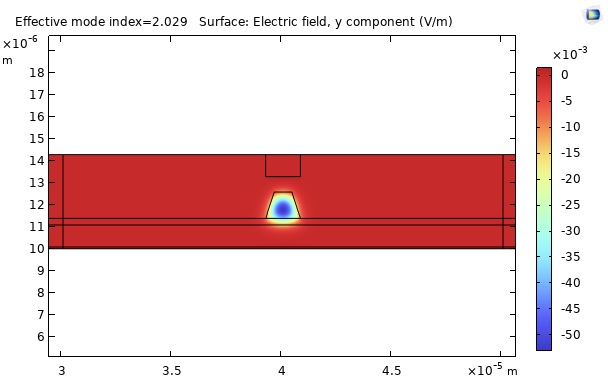
\includegraphics[width=0.7\linewidth]{ewfd-Ey-neff-2.029.png}
    %    \caption{Optical Field TE00 mode}
    %    \label{fig:ion_diffused_LN_wg}
    %\end{figure}
        
    %\begin{figure}
    %    \centering
    %    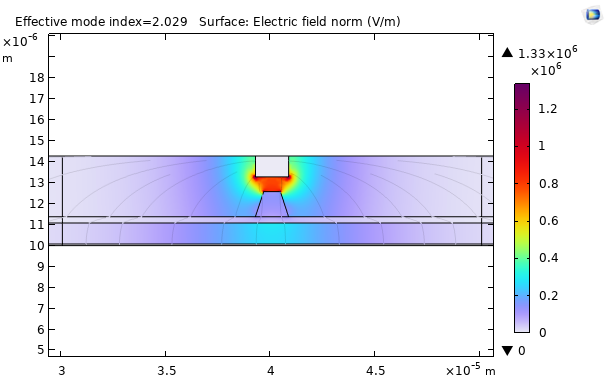
\includegraphics[width=0.7\linewidth]{es-Ey-neff-2.029.png}
    %    \caption{DC field distribution}
    %    \label{fig:rib-ridge_LN_wg}
    %\end{figure}

    In the table \ref{table:zhang-et-al}, calculated $V_{\pi}.L$ values and corresponding dimensions are given. In this work, $V_\pi L$ product is calculated to verify the simulation physics used and parameter configurations.
    
    \begin{table}[h]
        \centering
        \begin{tabular}{|c|c|c|c|}
            \cline{1-4}
            Geometry & Mode Index & Overlap & $V_\pi L$ \\ \cline{1-4}
            X-cut & 1.8872 & 0.5230 & 2.1679V         \\ \cline{1-4}
            Z-cut & 2.029 & 0.3516 &  2.4117V   \\ \cline{1-4}
        \end{tabular}
        \caption{Simulation results for X-cut and Z-cut Modulators}
        \label{tab:simulation-comparision}
    \end{table}

    In table \ref{tab:simulation-comparision}, the results of simulations, are done in this work, are seen. Mode index difference occurs due to different ridge height in two waveguide. As the ridge height decreases, wave will be more confined and the difference between mode index and material's refractive index increases. Also, large overlap value is result of having confinement in small region. 
    
    \begin{table}[h!]
        \centering
        \caption{$V_\pi L $ voltage comparision of this work with the ones obtained by Zhang et al. \cite{21}}
        \begin{tabular}{|c|c|}
            \hline
            X-Cut Modulator & Z-cut Modulator   \\
            \hline
            \begin{tabular}{c| p{1.85cm}}
                    %\hline
                    This Work & Paper
                    %\hline
                \end{tabular} & \begin{tabular}{c | p{1.5cm}}
                    %\hline
                    This Work & Paper \\
                    %\hline
                \end{tabular} \\
            \hline
            \begin{tabular}[t]{c c}
                    %\hline
                    2.1679\,V.cm & \;2.25\,V.cm 
                    %\hline
                \end{tabular} & \begin{tabular}{p{1.8cm} c}
                    %\hline
                    2.4117\,V.cm & 2.60\,V.cm \\
                    %\hline
                \end{tabular} \\
            \hline
            
        \end{tabular}
    \end{table}

    Zhang et al. \cite{21} has indicated that $V_{\pi}.L$ values in their paper are quantitative results for starting design of abovementioned geometries. This means values are not optimized. In the light of this information, percent error is calculated as 3.65\% in X-cut modulator and 7.24\% in Z-cut modulator. 

    \begin{figure}[h!]
        \centering
        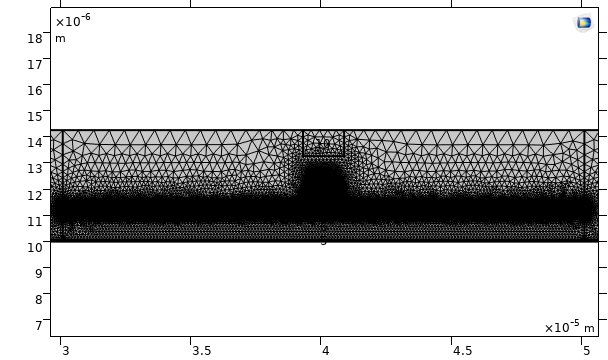
\includegraphics[width=0.50\linewidth]{optical-mesh.png}
        \caption{Optical mesh which COMSOL \textit{EM Wave Frequency Domain (ewfd)} generates} 
        \label{fig:optical-mesh}
    \end{figure}

    In Figure \ref{fig:optical-mesh} and \ref{fig:dc-mesh} measured meshes are seen. In order to precisely solve the domains where field modes confine, polygon definition is made and the region inside that polygon has more precise mesh.
    
    \begin{figure}[h!]
        \centering
        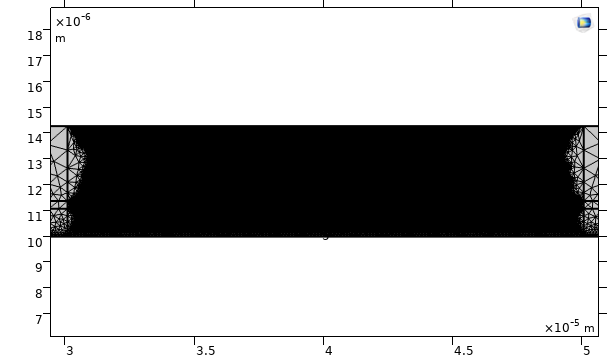
\includegraphics[width=0.50\linewidth]{dc-mesh.png}
        \caption{DC mesh which COMSOL \textit{Electrostatic (es)} generates} 
        \label{fig:dc-mesh}
    \end{figure}

    \subsubsection{Experimentally Verified $V_\pi$}

    Transmission characteristic of sample EO MZM is seen in Figure \ref{fig:experimental-pi} and measurement process was carried out by Girish Karthik. 

    \begin{figure}[h!]
        \centering
        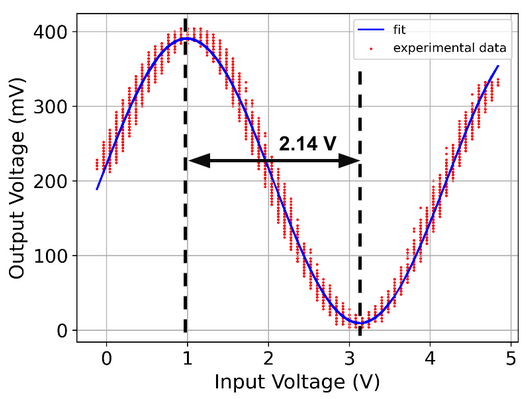
\includegraphics[width=0.55\linewidth]{girish_transmission_characteristic.PNG}
        \caption{Transmission characteristic of sample modulator with length of 0.920cm. Red dots represents experimental data which is sampled by oscilloscope.}
        \label{fig:experimental-pi}
    \end{figure}

    Since $V_\pi L $ voltage is constant and voltage and length of modulator is inversely propotional, 1-cm-modulator has smaller voltage value which is seen in Table \ref{tab:experimental-comparision}. Percent error between experimental and simulation data is 29.7\%.
    
    \begin{table}[h]
        \centering
        \begin{tabular}{|c|c|c|c|}
            \cline{1-4}
            Method & Mode Index & Overlap & $V_\pi L$ \\ \cline{1-4}
            Realized Measurement & - & - & 1.969\,V.cm         \\ \cline{1-4}
            Simulation & 1.9125 & 0.2598 &  2.8301 \,V.cm   \\ \cline{1-4}
        \end{tabular}
        \caption{Experimentally measured $V_\pi L$ value and its simulation results}
        \label{tab:experimental-comparision}
    \end{table}


    
    \subsubsection{Parametric Sweep In X-cut Modulator - $V_\pi L $ And Top $SiO_2$ Layer Dependence}

    Thickness change of top layer silica has effect on the overlap integral. As the microwave electrodes moves away from optical waveguide, overlap integral decreases. This effect can be seen on the figure \ref{fig:voltage-top-silica-dependence}. 
    
    \begin{figure}[h]
        \centering
        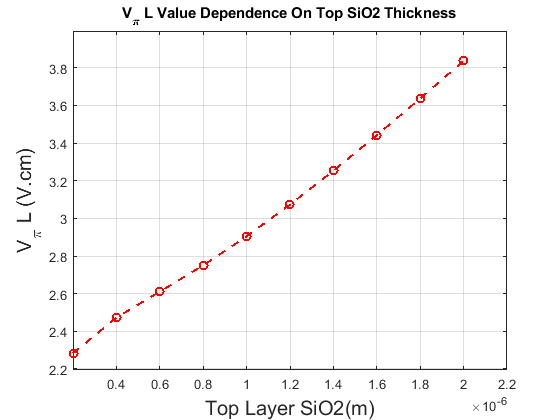
\includegraphics[width=0.75\linewidth]{overlap_updated_v_piL-top_sio2.png}
        \caption{In x-cut EO MZM, top layer silica has changed and reduced }
        \label{fig:voltage-top-silica-dependence}
    \end{figure}

    In order to have small $V_\pi$ value, one can think to place the electrodes as close as possible to optical waveguide. However, plasmonic behavior start to arise in that case since metal-dielectric boundary becomes easily available for the optical wave and optical confinement is not achieved. This effect is seen in figure \ref{fig:x-cut-plasmonics}.

    \begin{figure}[h]
        \centering
        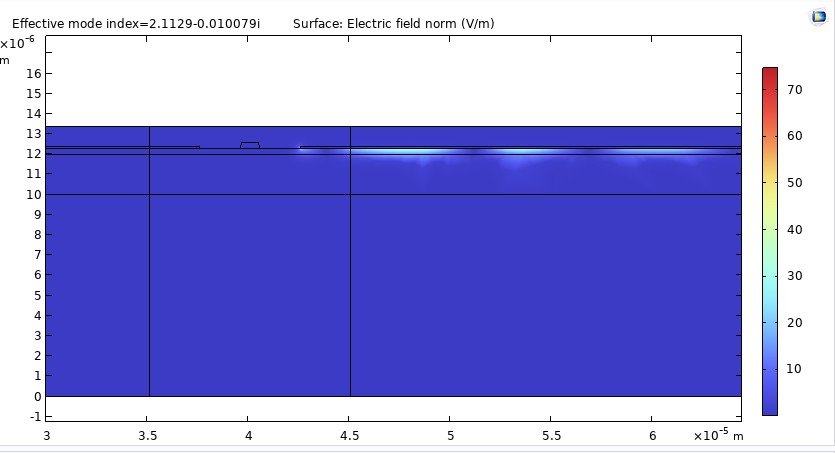
\includegraphics[width=0.7\linewidth]{loss_try.PNG}
        \caption{Plasmonic behavior in metal-LN interface. Silica layer is removed in this case.}
        \label{fig:x-cut-plasmonics}
    \end{figure}

    The top silica layer helps preserve optical confinement and the overlap integral, preventing degradation that would otherwise increase optical loss 

    \begin{figure}[h]
        \centering
        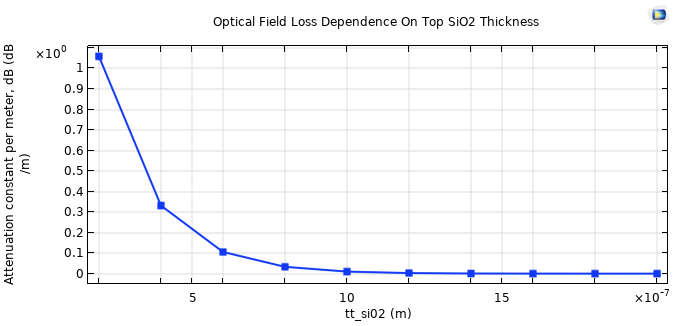
\includegraphics[width=0.75\linewidth]{x-cut-tt_sio2 loss.png}
        \caption{In x-cut EO MZM, top layer silica (x-axis) has parametrically changed and corresponding loss values are observed.}
        \label{fig:x-cut-tt_sio2-loss}
    \end{figure}

    As it is seen on figure \ref{fig:x-cut-tt_sio2-loss}, if the metalic electrodes are close to optical waveguide losses (dB/m) will increase. Critical observation would be the speed of change, it can be represented in linear scale, instead of logarithmic one. However, it is still undesirable.
    
    \subsubsection{Parametric Sweep In X-cut Modulator - $V_\pi L $ And Coplanar Waveguide Gap Dependence}

    Another approach to increase overlap between optical and microwave fields is having smaller gap between coplanar waveguide signal and ground electrodes. 
    
    \begin{figure}[h!]
        \centering
        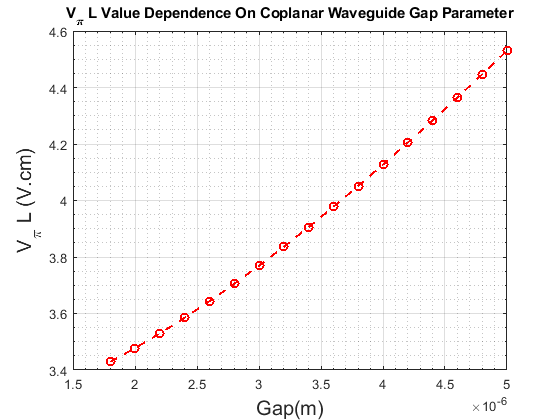
\includegraphics[width=0.73\linewidth]{overlap_updated_v_piL_cpw_gap.png}
        \caption{In x-cut EO MZM, gap between microwave electrodes has parametrically swept.}
        \label{fig:voltage-gap-dependence-x-cut}
    \end{figure}

    \newpage
    
    $V_\pi L$ value change almost linearly with respect to gap parameter in figure \ref{fig:voltage-gap-dependence-x-cut}. Also, plasmonic effects still persist. This requires loss analysis for optical mode. In figure \ref{fig:x-cut-gap-loss}, change of loss in response to gap change is fast and small in amplitude. Increasing distance may decrease loss however it degrades $V_\pi$ voltage. 
    
    \begin{figure}[h]
        \centering
        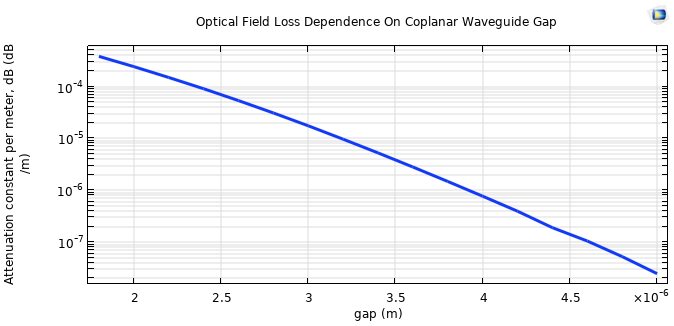
\includegraphics[width=0.75\linewidth]{xCut Loss vs gap change.png}
        \caption{In x-cut EO MZM, change of gap and its effect on optical loss is seen. Vertical scale is logarithmic.}
        \label{fig:x-cut-gap-loss}
    \end{figure}
    
    \subsubsection{Parametric Sweep In Z-cut Modulator - $V_\pi L$ And Top $SiO_2$ Layer Dependence}

    Z-cut modulators have different microwave electrode orientation due to the reason mentioned in Optical Waveguides section. In this configuration top silica layer thickness has crucial effect on overlap integral and overall performance of the device. 

    \begin{figure}[h]
        \centering
        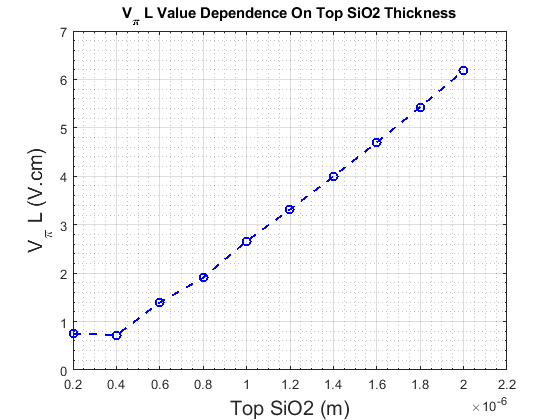
\includegraphics[width=0.75\linewidth]{overlap_integral_updated_2nd_neff_without voltage selection.png}
        \caption{In z-cut EO MZM, change of top silica layer and $V_\pi L$ value relation is seen.}
        \label{fig:voltage-thickness-dependence-z-cut}
    \end{figure}

    \newpage

    For a proper comparision, x-cut and z-cut modulators have both same top silica sweeps. However, z-cut modulator does not works properly for 200nm and 400nm top silica thicknesses because electrode overlaps with optical waveguide, which leads to unrealizable geometry. This result is seen in figure \ref{fig:voltage-thickness-dependence-z-cut}. Considering $V_\pi L$ values starting from 600nm, they are almost linearly dependent on top silica thickness.

    As for optical loss in z-cut modulator, it is drastically affected from top silica thickness. In figure \ref{fig:z-cut-tt_sio2-loss}, vertical scale indicates loss (dB/m) and it is represented in logarithmic scale. 

    \begin{figure}[h]
        \centering
        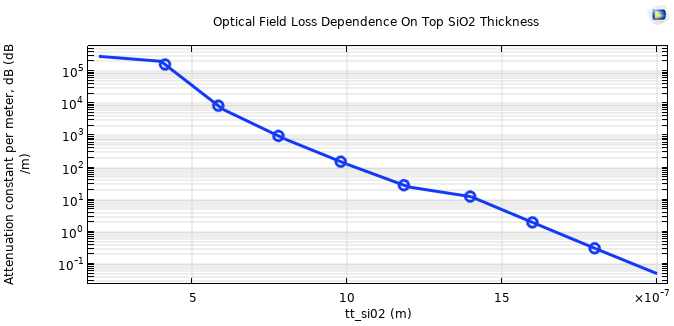
\includegraphics[width=0.75\linewidth]{z-cut loss analysis.png}
        \caption{In z-cut EO MZM, change of top silica layer has strong impact on optical loss}
        \label{fig:z-cut-tt_sio2-loss}
    \end{figure}
    
    For this large loss value, optical field does not confine in nonlinear medium, as in figure \ref{fig:enter-label} and overlap integral degrades. Moreover, this unconfined mode supports the profitless $V_\pi L$ voltages for 200nm and 400nm in figure \ref{fig:voltage-thickness-dependence-z-cut}. 

    \begin{figure}[h]
        \centering
        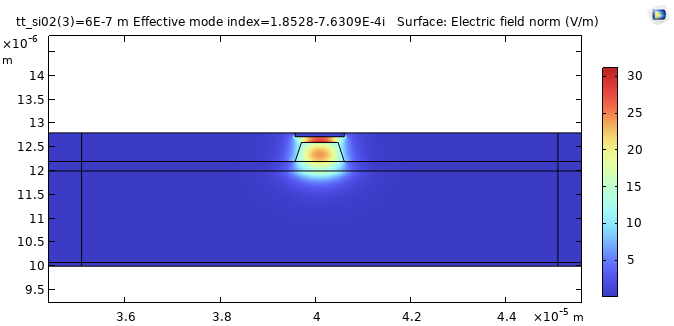
\includegraphics[width=0.75\linewidth]{z-cut confinement issue.png}
        \caption{Due to severe loss, optical mode does not confine in z-cut modulator}
        \label{fig:enter-label}
    \end{figure}
